%&latex
\chapter{CASP-7}
\label{chapter:casp}

\begin{quote}
``Today we may face some boring task or idle conversation that feels like a complete waste of time. 
Perhaps next week or next year we'll understand that nothing is wasted. That is the economy of our 
universe; even a weed is simply a flower whose use has yet to be discovered.'' \\
--- \textit{Mort Crim}
\end{quote}

\section{Introduction}

\casp-7 stands for the \xth{7} Critical Assessment of Protein Structure Prediction. \casp, which was introduced in section \ref{section:prot_model:casp} as a community-wide competition for protein structure prediction, has taken place every two years since 1994.
Throughout \casp-7, a total of 22,670 primary predictions were received from 253 unique groups. \casp-7 also presented the largest number of target structures to date, exceeding 100 for the first time.

\prearcus\ was still in development at the beginning of \casp-7, meaning that only targets released following the 21\superscript{st} June
could be attempted.
In addition to this, only target structures smaller than 250 amino acids were considered, as larger proteins contain a prohibitive number of atoms when evaluated under \gbsa\ -- Such multi-body calculations are expensive and were in excess of the amount of computer power which was available at the time. Finally, only structures which had one or more structural templates of better than approximately 24\% sequence-identity were attempted; commonly referred to as the template-based modelling category. It was expected that only those targets with approximately \textgreater40\% sequence identity would yield models of high quality, as the level of structural divergence below this cut-off would be too great for the use of rigid-core modelling.  Following these constraints, a total of seven targets were selected and are listed in table \ref{table:casp:targets}.
For the purposes of discussion, two of these selected targets had only low sequence-identity structural templates.

\begin{table}[htbp]
\begin{center}
\begin{tabular}{+c^c^c^c^c^c}
\toprule
\rowstyle{\bfseries}
 \multirow{2}{*}{Target ID} & \multirow{2}{*}{Name} &  \multirow{2}{*}{N\subscript{res}} & Target & Template & Sequence \\
\rowstyle{\bfseries}
  &  &  & PDBID & PDBID & Identity \\
\midrule
T0340 &  SLC9A3R2A  & 90 &   2HE4 &     1G9OA &    60\% \\
T0345 &  GPX2    & 185 &  2HE3 &     2F8AA &    68\% \\
T0346 &  PPI63   & 172 &  2HE9 &     2GW2A &    56\% \\
T0359 &  MPDZ3   & 97  &  2IWN  &    2FNEA &    40\% \\
T0366 &  MPDZ12  & 106 &  2IWO or 2IWP &     2FNEA  & 42\% \\
T0374 &  APC5605 & 160 &   2I6C &   1YR0A &    24\% \\
T0379 &  PG0725  & 208 &   2I6X &   2B0CA &    25\% \\
\bottomrule
\end{tabular}
\caption{The \casp-7 targets predicted during this work.}
\label{table:casp:targets}
\end{center}
\end{table}

Due to the limited number of  viable candidates chosen from those available in \casp, there were insufficient data to perform a full quantitative analysis.
The overall aim of this chapter is, therefore, to give a \emph{qualitative} overview of the strengths and weaknesses of the primary models produced by the method outlined by chapters \ref{chapter:reduced_rep} and \ref{chapter:prearcus}.
The purpose of this analysis was primarily to identify potential shortcomings in the method developed to this point. A full quantitative analysis of the abilities of \prearcus\ is instead conducted in chapter \ref{chapter:methods}; validated against other loop modelling methods using a far more comprehensive in-house data-set.

\section{The Modelling Procedure}

The following section outlines the modelling process developed for the \casp-7 competition. In general, typical comparative modelling procedures were followed, using standard tools where appropriate. First of all, in this section rigid-core selection is discussed in relation to structural examples.\ This is followed by a discussion of the information gained from multiple-sequence alignments. Finally, the method by which loops were selected for \abinitio\ construction under \prearcus\ is discussed.

\subsection{Initial Model Structure Selection}

As \prearcus\ is fundamentally intended as a sub-component of the comparative modelling process, it is intrinsically incapable of building whole-protein models. However, high-quality initial rigid-core structures were required for each \casp-target prior to the testing of \prearcus. As part of \casp\ itself, a number of automated protein modelling servers are queried for every \casp\ target. The best five models are then automatically provided by each server and made publicly available well before the submission deadline for other predictions. As these models are produced automatically, usually from multiple structural template alignments, the completed server models provide an ideal foundation to blind-test \prearcus.
It is noteworthy that the automated servers are designed to facilitate high-throughput modelling outside of \casp; they, therefore, may not produce the highest quality predictions possible if more resources were allocated to the modelling of specific sections. Such a \emph{concentrated} structural-refinement is the task of \prearcus.

The chosen procedure involved the initial energy minimisation of server models under the standard  \prearcus\ stage 3 Cartesian forcefield, defined previously in section \ref{section:prearcus:stage3_refinement}. For every prediction server against every \casp-7\ target, the best model (as ranked by the server-method itself) was energy minimised. The structure with the lowest energy was selected to be the rigid-body for use by \prearcus. An example range of minimised \ambergbsa\ energies for T0345 are shown in table \ref{table:casp:target_ene}.

\begin{table}[htbp]
\begin{center}
\begin{tabular}{+c^c^c^c}
\toprule
\rowstyle{\bfseries}
 Rank & Competitor & Model \# & Minimised Energy  \\
\midrule
\first & \textsc{Robetta} & 1     &     -3313.341 \\
\second & \textsc{Protinfo-AB}   & 1&   -3305.885 \\
\third & \textsc{Raptoress}    & 1&    -3305.036 \\
\xth{4} & \textsc{Loopp}  & 1&  -3303.977 \\
\xth{5} & \textsc{NN\_PUT\_lab}   & 1&    -3303.977 \\
\xth{6} & \textsc{Protinfo}    & 1&     -3301.677 \\
\bottomrule
\end{tabular}
\caption[An example minimised-energy profile for the best six T0345 server models.]{An example minimised-energy profile for the best six T0345 server models. As the \textsc{Robetta} server produced the lowest energy model, this structure was chosen as the rigid-core model for \prearcus\ loop construction.}
\label{table:casp:target_ene}
\end{center}
\end{table}

\subsection{Server Model Structural Similarity}

Before discussing the structural nature of the automated-server models, this section begins by briefly presenting one of the target \xray\ structures, which of course was not publicly available when the \mbox{\casp-7} predictions were undertaken.
In an interesting coincidence, T0366 was crystalised independently by two separate groups. Both groups released PDB entries, being 2IWO and 2IWP, which resolved to 1.70\AA\ and 2.15\AA\ resolution respectively. For general interest, both structures are shown here in figure \ref{fig:casp:crystalsimilarity}. As one would expect and hope, the two structures are highly similar, but with some interesting small differences; most likely due to the exact crystal packing environment. The two structures align with a 0.38\AA\ RMSD to each other over all \ca-atoms, with most pronounced difference at the C-terminus and one surface loop.

\begin{figure}[hbtp]
\begin{center}
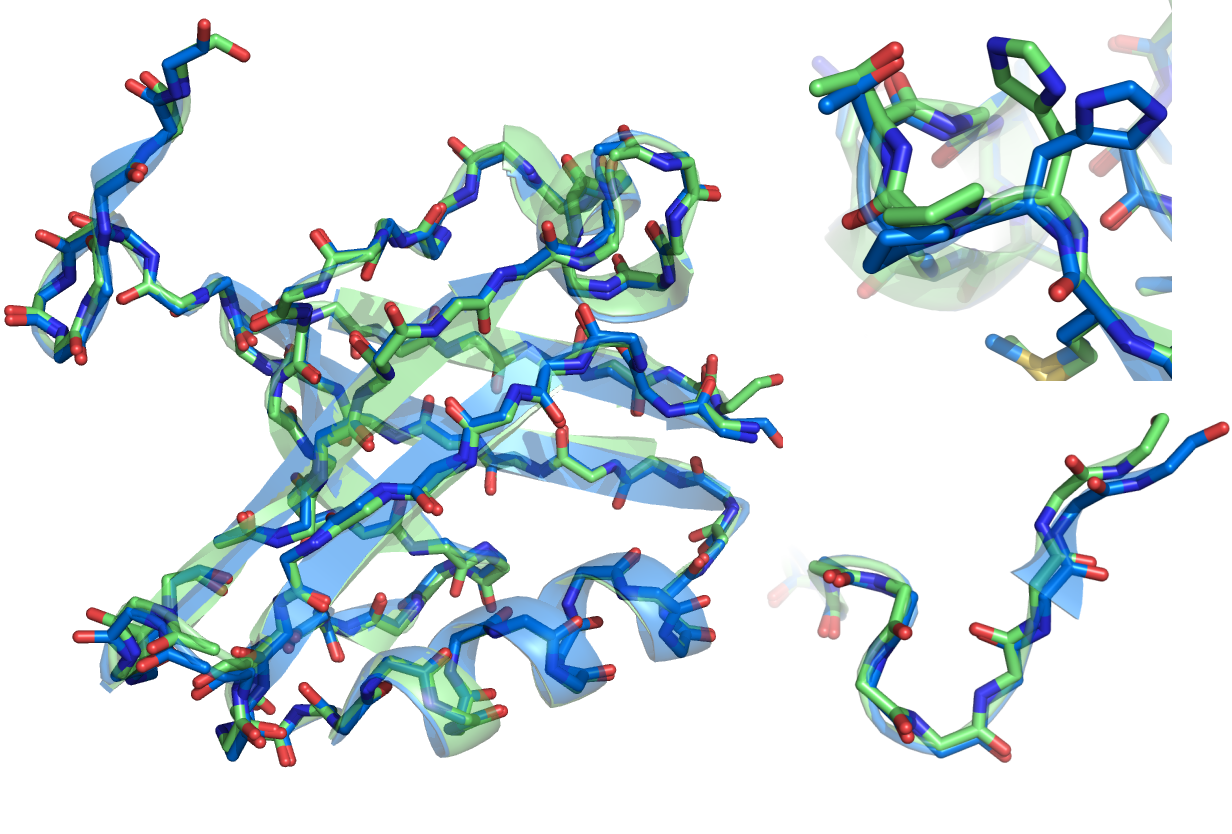
\includegraphics[width=0.95\textwidth]{07-CASP/crystal_similarity/crystal_similarity.png}
\caption[Same-sequence \xray\ structure similarity]{Same-sequence \xray\ structure similarity. Structures of 2IWO and 2IWP are shown in blue an green respectively. On the right of the figure, zoomed sub-images of a deformed loop and the C-terminus are shown.}
\label{fig:casp:crystalsimilarity}
\end{center}
\end{figure}

With this in mind, the four lowest-energy server predictions for T0366 are shown in figure \ref{fig:casp:serversimilarity}. It can be seen that the server predictions have more structural similarity to each other than the crystal structure; in essence, due to their high structural similarity to the same  chosen templates. These aspects were described previously in section \ref{section:comparative_modelling}, as a common undesirable feature of comparative models, where structural refinement remains a significant issue.
In this figure, it can clearly be seen that, as expected, there is a greater structural diversity between models in the surface loops. As the target sequence has only 42\% sequence identity to the closest structural template, this level of deviation is within expected values, as there is little or no homology information available for these regions. It is these divergent surface loops which are given to \prearcus\ for attempted refinement.
In addition, the C-terminus is essentially undefined, as all server models are in complete disagreement as to its location. 

\begin{figure}[hbtp]
\begin{center}
\subfigure[Rigid-body only]{
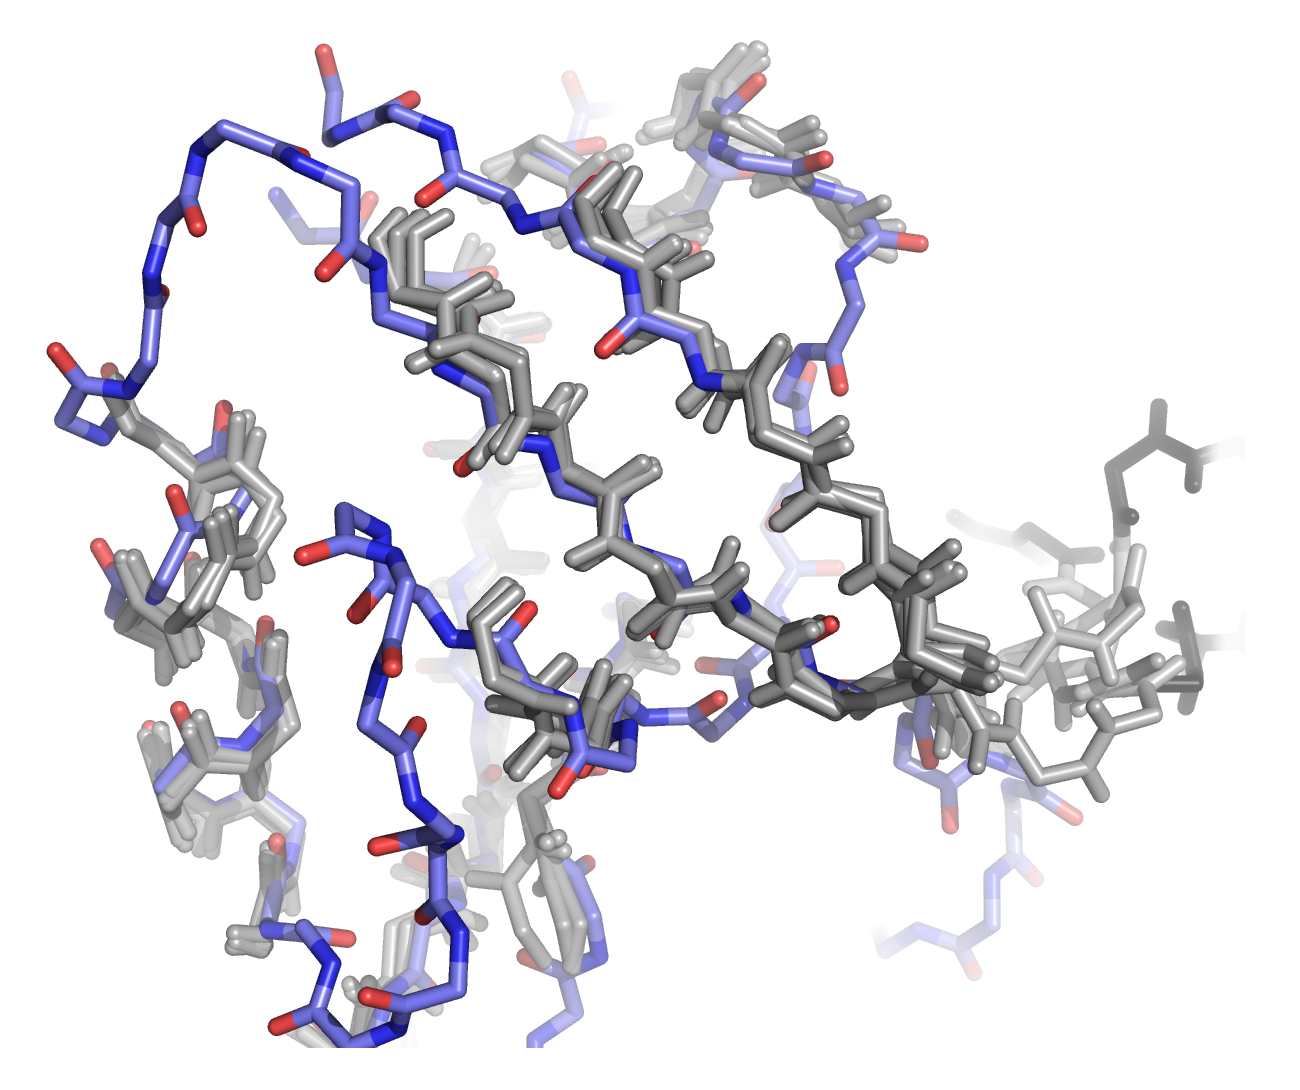
\includegraphics[width=0.75\textwidth]{07-CASP/template_similarity/core.png}}
\subfigure[Rigid-body plus two surface loops]{
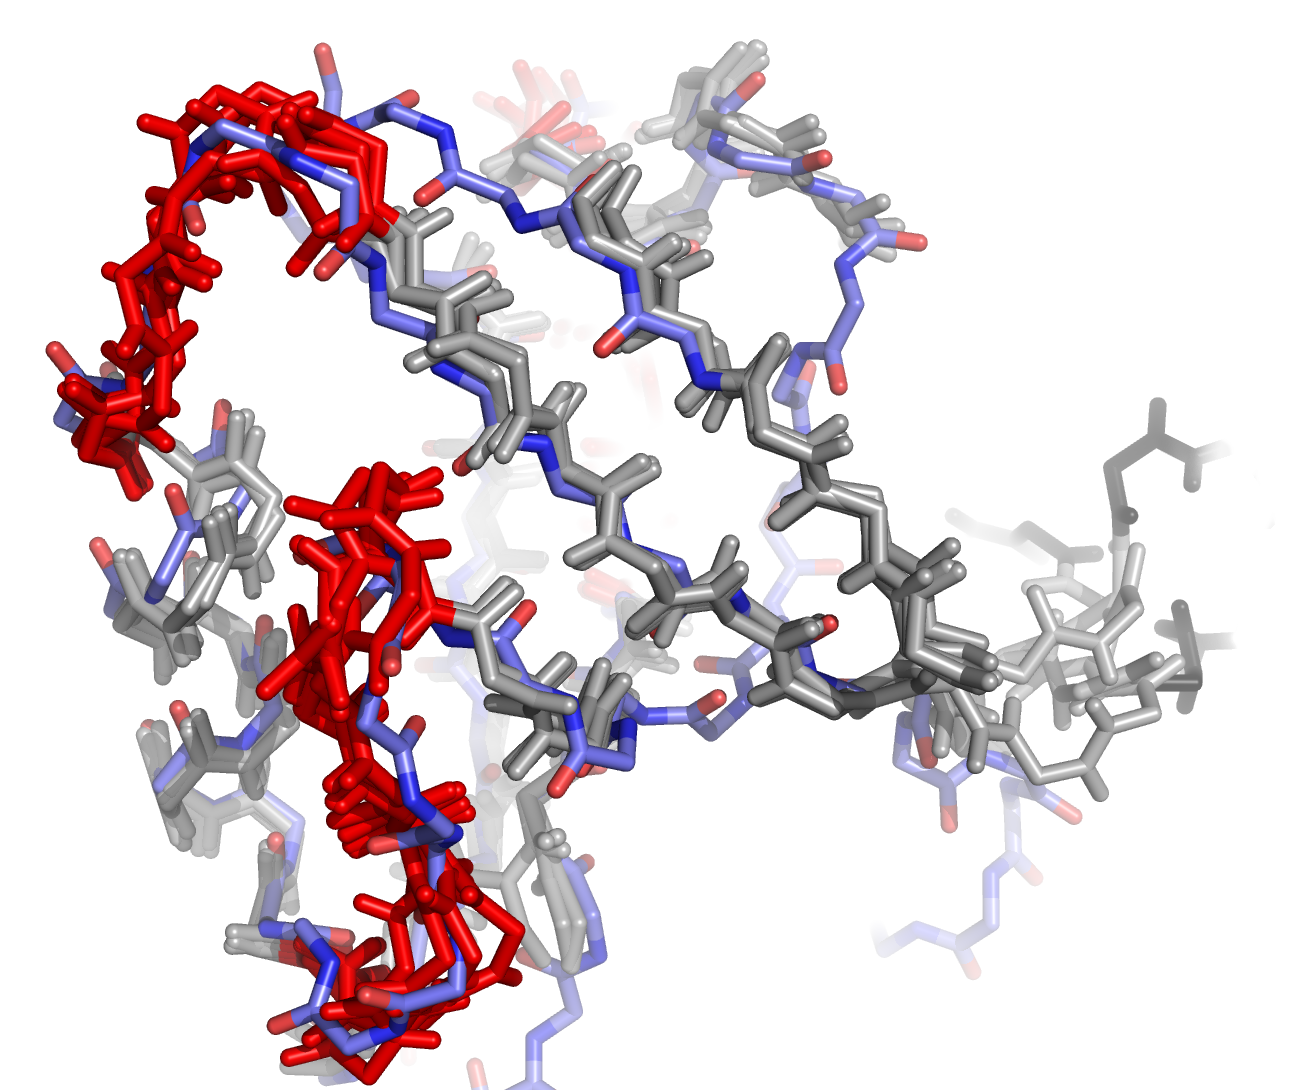
\includegraphics[width=0.75\textwidth]{07-CASP/template_similarity/core_plus_twoloop.png}}
\caption[Server-model similarity]{Server-model similarity. The crystal structure (2IWOA, 1.7\AA\ resolution) for T0366 is shown in blue. In sub-figure a), only the conserved protein core is shown in grey for selected low-energy server models. It can be seen that there is no consensus as to the conformation of the C-terminus. In sub-figure b), two surface loops are introduced to illustrate the increased structural uncertainty in these regions.\ This is demonstrated by the increased disagreement between models as to the precise conformation.}
\label{fig:casp:serversimilarity}
\end{center}
\end{figure}

\subsection{Multiple Sequence Alignment}
\label{section:casp:seq_ali}

In order to gain insight from sequence information, the sequences of the \casp-7\ targets were submitted to the \textsc{ExPASy BlastP} server. This server can be requested to query any candidate sequence against only those sequences in the PDB using \textsc{PsiBlast}\cite{SEQUENCE:PSIBLAST} and then to perform a multiple sequence alignment using the \textsc{ClustalW} algorithm\cite{SEQUENCE:CLUSTALW}.
\subsection{Loop Selection}

Loop selection was performed primarily using the \dssp-based definition which was developed for \thothloopdb\ in section \ref{section:loopcriterion}. This used the \dssp\ file produced from the chosen, complete, template server model. As these are models, with reduced structural certainty, in some cases the loop regions were manually extended using human judgement. This was only performed if either  significant  structural disagreement was found between the low-energy server templates, or there was no local sequence-similarity when comparing multiple template-PDB \mbox{sequence$\to$structure} relationships (obtained from the multiple sequence alignment described in section \ref{section:casp:seq_ali}).

Each loop was re-modelled separately, where prior to each loop simulation, any existing coordinates from the server model were discarded. The  loop structure with the lowest energy for the complete protein was selected for use in the final refined model. Where steric conflicts existed between refined loops, which was rare, the loop which resulted in the higher energy structure was replaced with its second best energy conformation. This was repeated until no steric conflict was present.


\section{Results}

Table \ref{table:casp:targets} showed that models were chosen with a wide variety of maximal sequence-identities to their closest structural template.
In light of this, the discussion here divides into three categories based upon on high, medium and low sequence identity, defined here as approximately  \textgreater60\%, \textgreater40\% and \textgreater20\% respectively.

\subsection{High and Medium Sequence-Identity}

  A high sequence-identity template was available for T0345 with 68\% identity to the candidate sequence. In total, the prediction of nine loops for T0345 was attempted, with varying accuracy. The exact RMSD values are shown in table \ref{table:casp:T0345rmsd}. More specific structural aspects are discussed in the remainder of the section. In general, however, it can be said that the predictions were of good structural quality. The best three were under 25\degree\ \arms\ and so can be said to reside within the correct Ramachandran regions. Some others, although showing low Cartesian RMSD values, compare less favourably in torsional space.

\begin{table}[htbp]
\begin{center}
\begin{tabular}{+c^c^c^c^c^c}
\toprule
&&\multicolumn{3}{c}{\textbf{\crms\ Type}}&  \\
\rowstyle{\bfseries}
 Start & \multirow{2}{*}{Length} & \ca & Heavy-atom & Torsional & Figure \\
\rowstyle{\bfseries}
 Residue && (\AA) & (\AA) & (degrees) & Reference \\ 
\midrule
157  &   6   &    0.97  &  1.35  &  14.27 & -- \\
74   &   7   &    0.87  &  1.82  &  14.94 & \ref{fig:casp:t0345_best} (\ref{fig:casp:t0345_rama}-a)\\ 
167  &   8   &    1.08  &  2.33  &  22.07 & -- \\
54   &   7   &    1.20  &  2.11  &  47.35 & -- \\
122  &   8   &    1.26  &  3.59  &  52.70 & -- \\
20   &   7   &    2.75  &  4.32  &  58.56 & -- \\
12   &   5   &    2.08  &  2.61  &  59.37 & -- \\
94   &   7   &    1.72  &  4.30  &  59.54 & \ref{fig:casp:t0345_worst} \\
34   &   6   &    1.07  &  1.42  &  71.22 & \ref{fig:casp:t0345_poor} (\ref{fig:casp:t0345_rama}-b) \\
\bottomrule
\end{tabular}
\caption[Prediction]{Prediction RMSD values for \casp-target T0345.
Data is sorted by \arms\ over the three \mainchain\ torsions.}
\label{table:casp:T0345rmsd}
\end{center}
\end{table}

One of the most successful loop predictions for T0345 is shown in figure \ref{fig:casp:t0345_best}. The structure is presented following rigid-body superimposition, \emph{not} loop superimposition. Minor Cartesian displacement occurs along the entire length of the loop. However, as this minor deformation begins at the C-terminal anchor region, which does not move during simulation, a 100\% accurate prediction was impossible. This means that, in hindsight, the selected loop region should have been very slightly larger; although, the deviation in this case is very minor. From the Ramachandran plot shown in \mbox{figure \ref{fig:casp:t0345_rama}-a}, it can be seen that all the residues are in the correct regions with most residues extremely close to their experimental values.
If the \mainchain\ deformation is considered, then five of the seven \sidechain\ conformations are predicted correctly, with essentially correct \Chi-angles.


\begin{figure}[hbtp]
\begin{center}
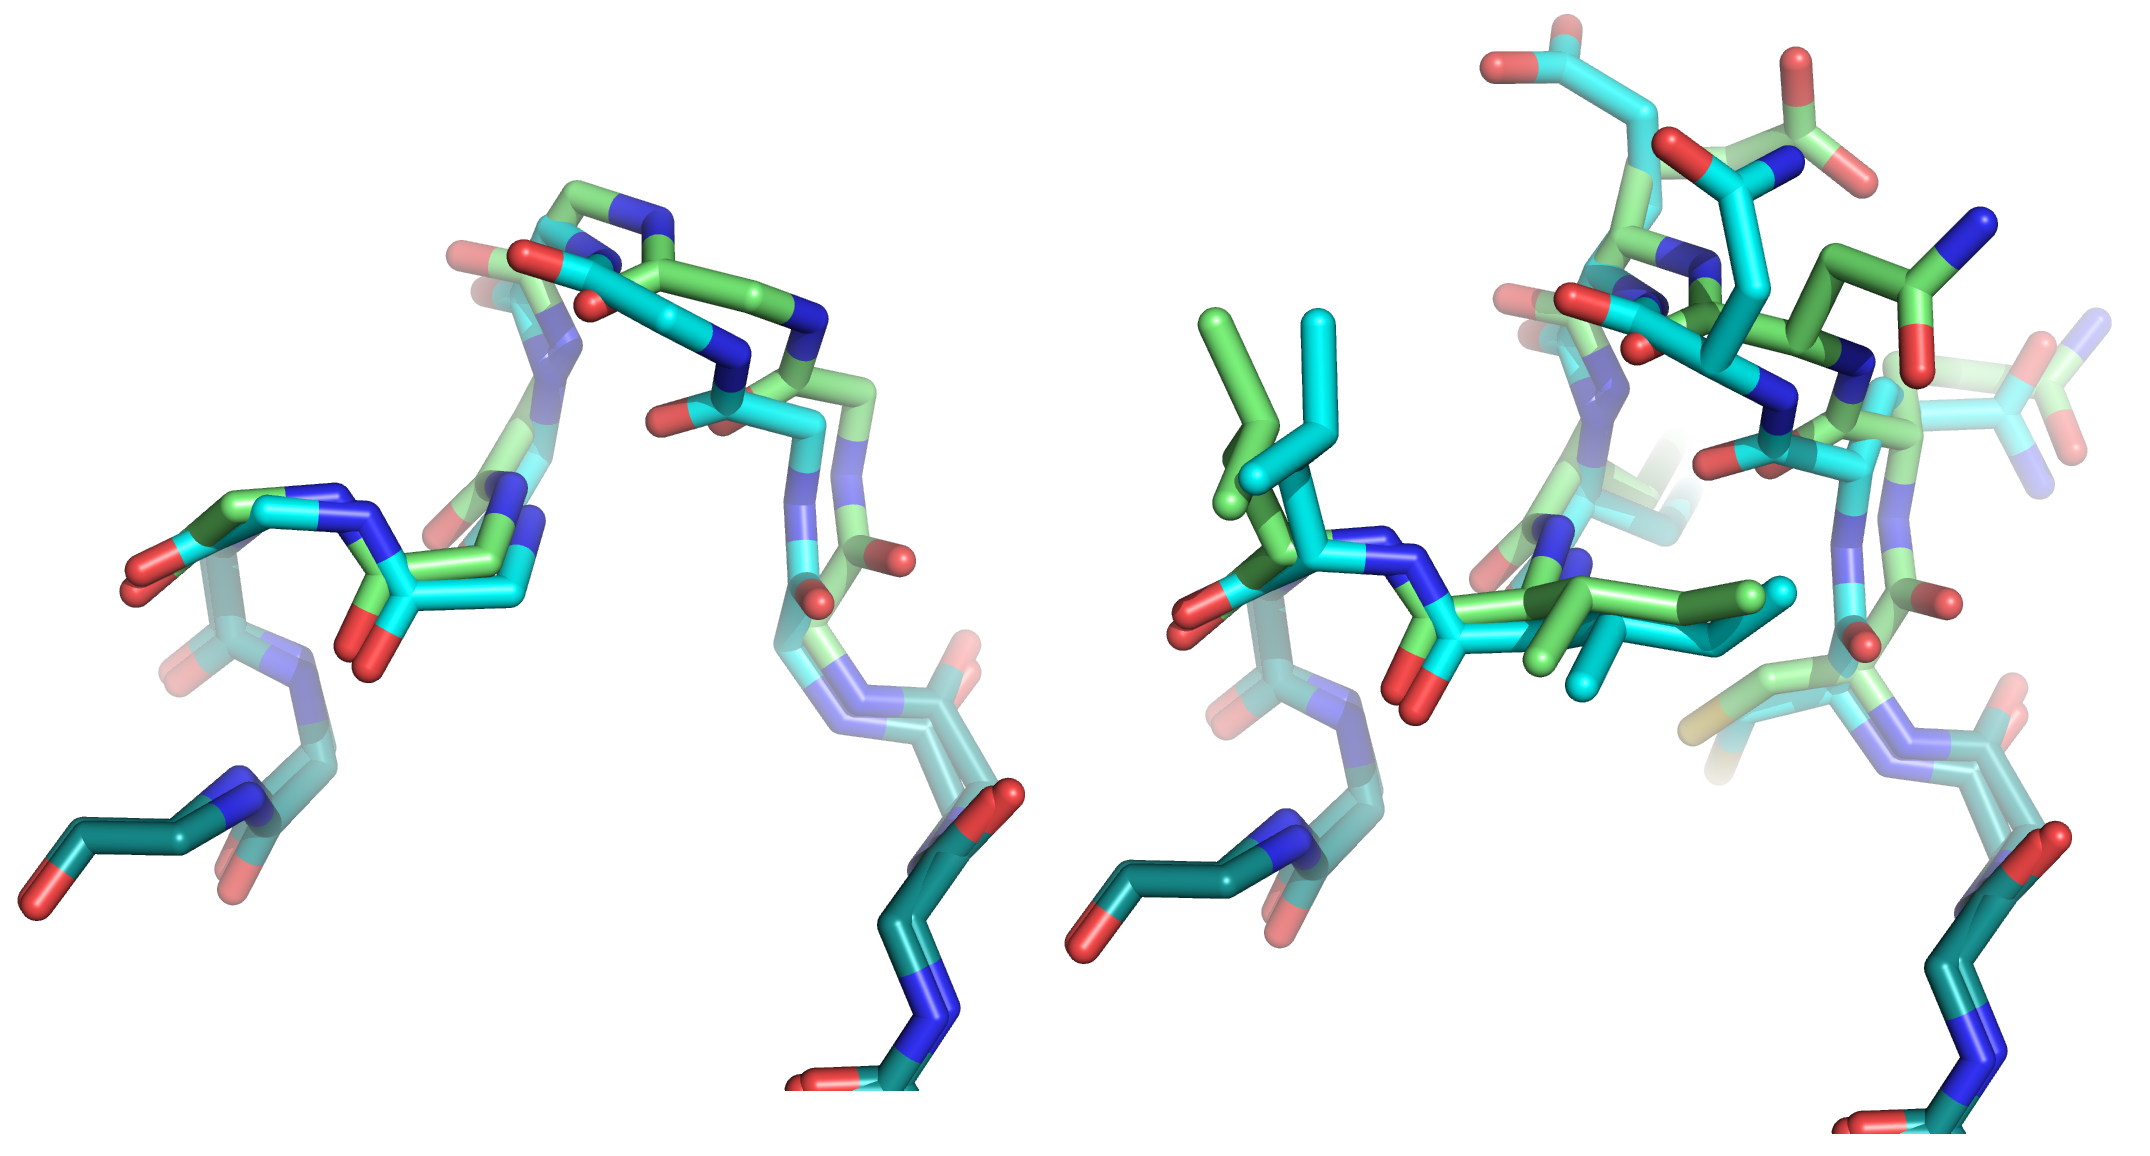
\includegraphics[width=0.75\textwidth]{07-CASP/high-t0345/best_pred_74_7.png}
\caption[One of the most successful predictions from T0345]{One of the most successful predictions from T0345; a \mer{7} loop beginning at residue Cys-74. The loop is shown on the left with no \sidechains\ for increased clarity. The crystal structure, model structure and anchor residues are shown in green, cyan and dark cyan respectively.}
\label{fig:casp:t0345_best}
\end{center}
\end{figure}


\begin{figure}[hbtp]
\begin{center}
\subfigure[For the structure in figure \ref{fig:casp:t0345_best}]{
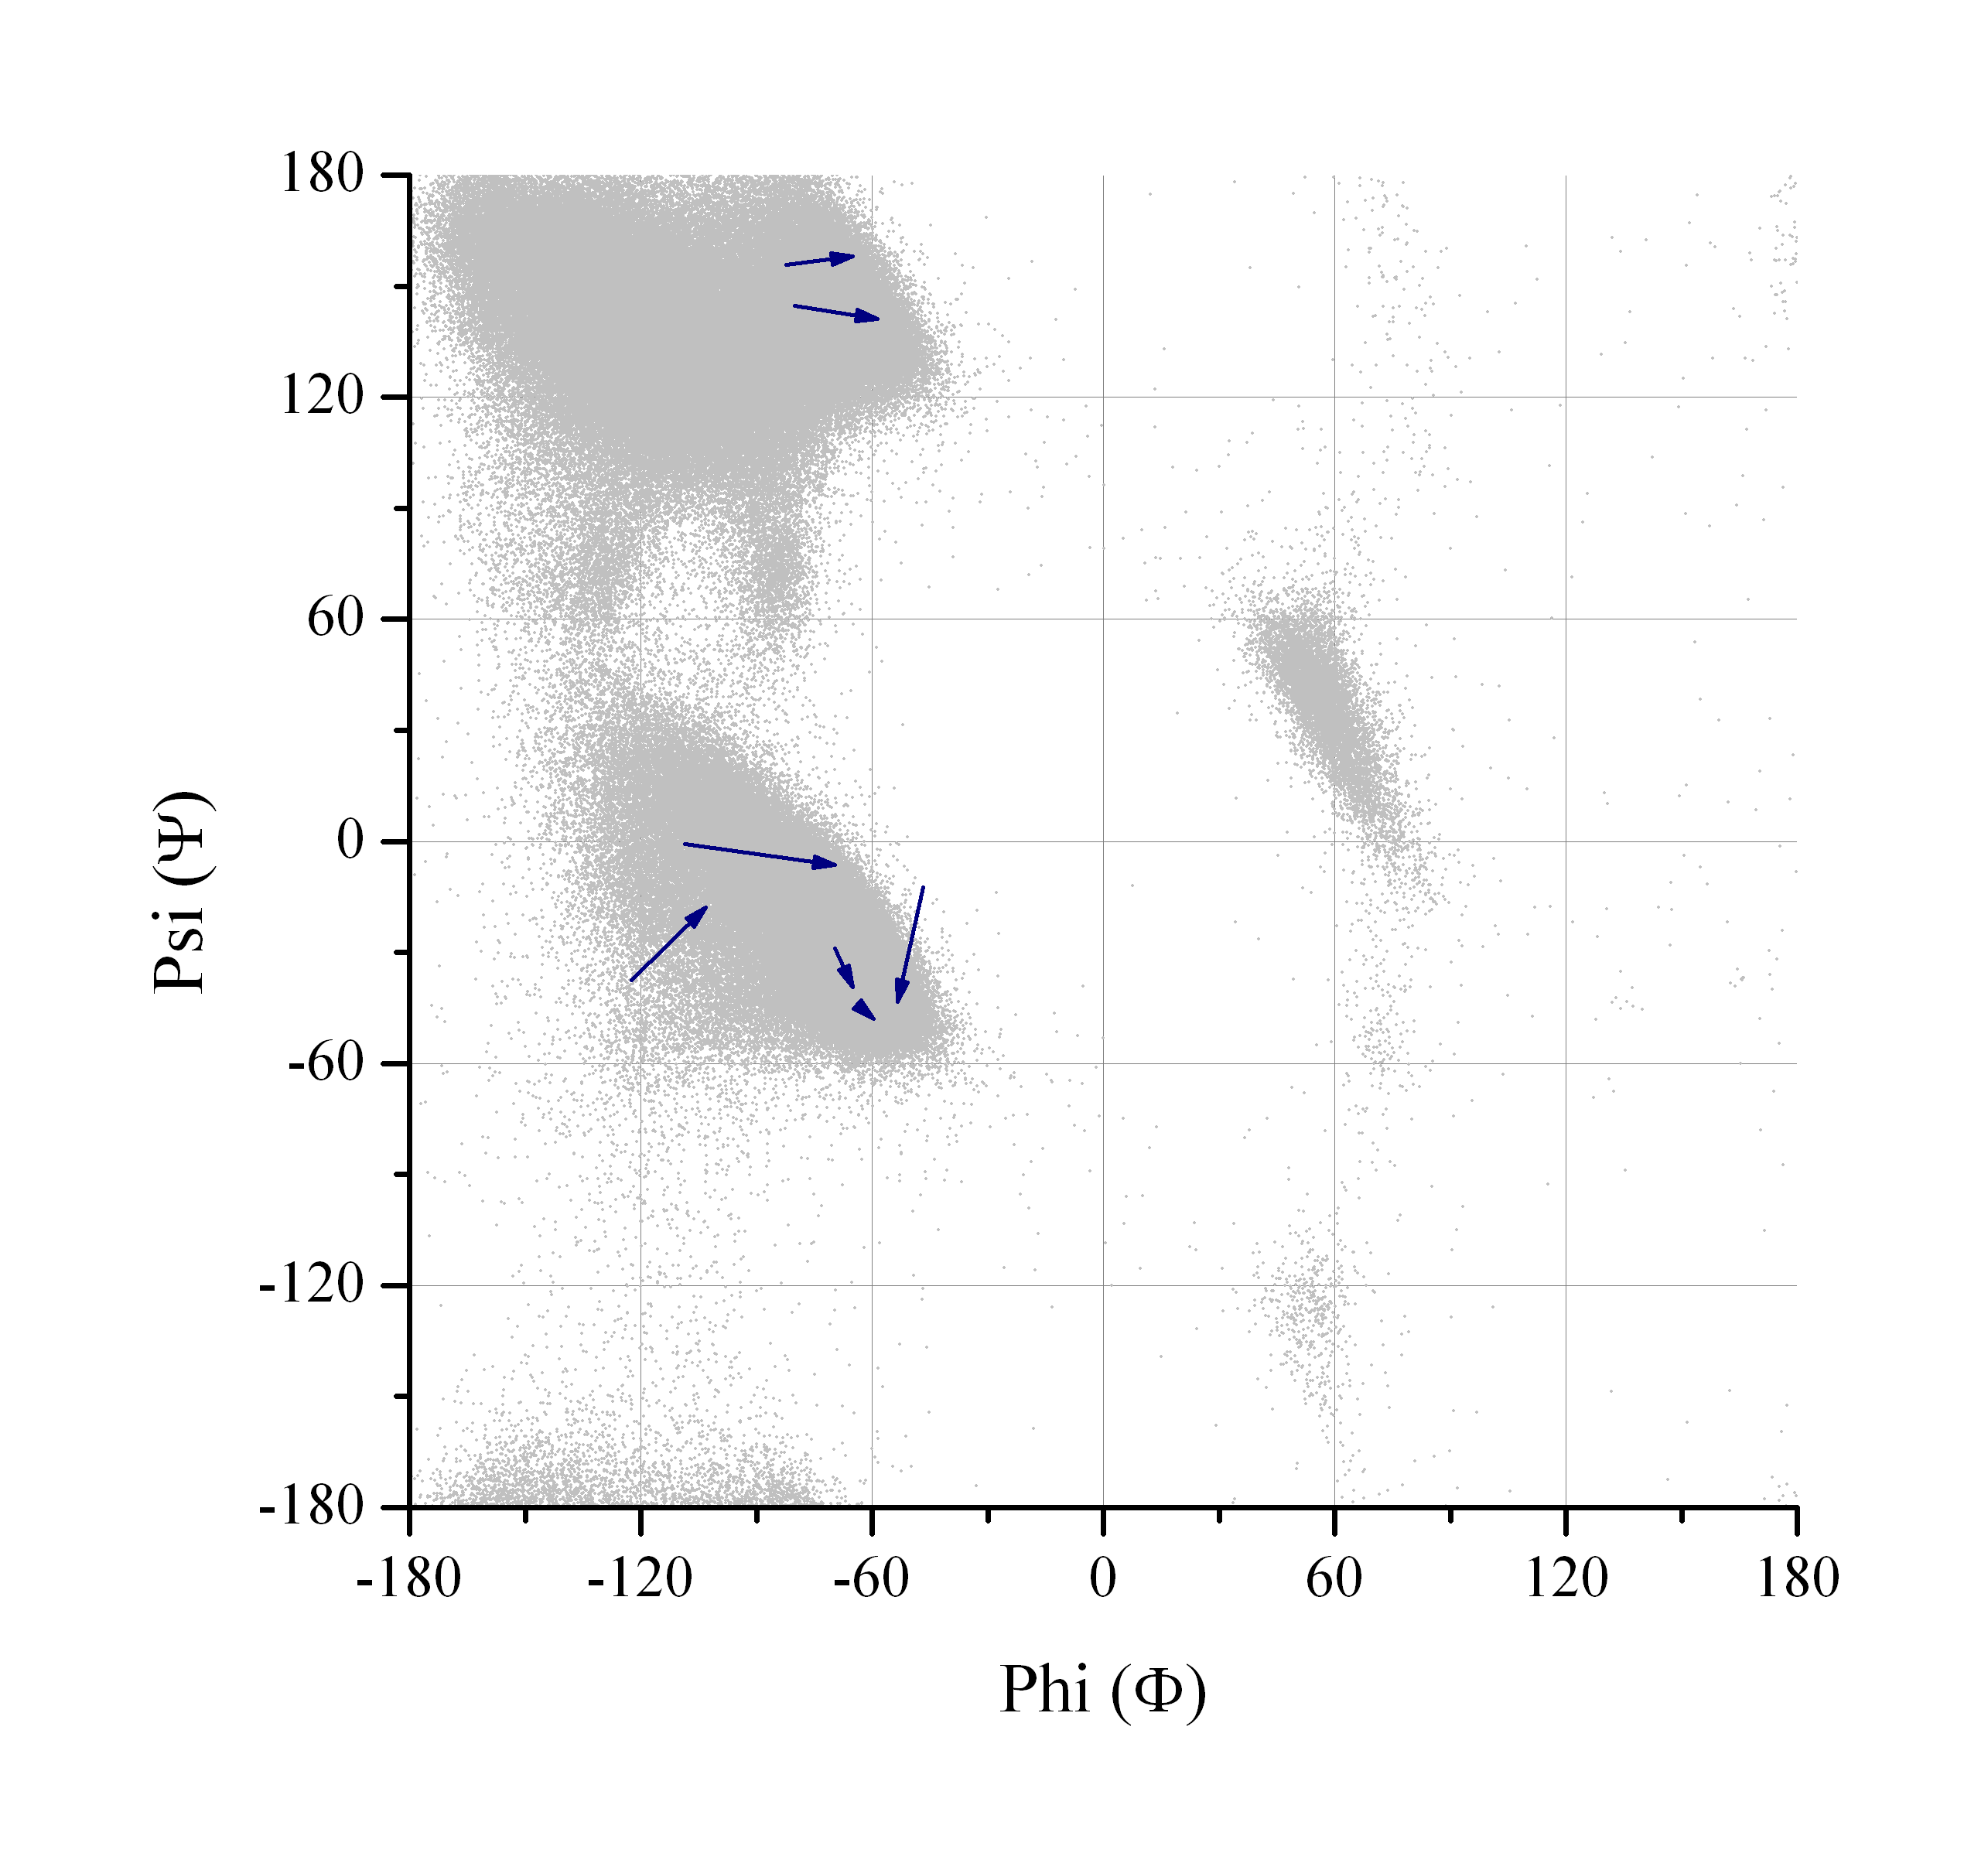
\includegraphics[width=0.45\textwidth]{07-CASP/high-t0345/best_pred_74_7_rama.png}}
\subfigure[For the structure in figure \ref{fig:casp:t0345_poor}]{
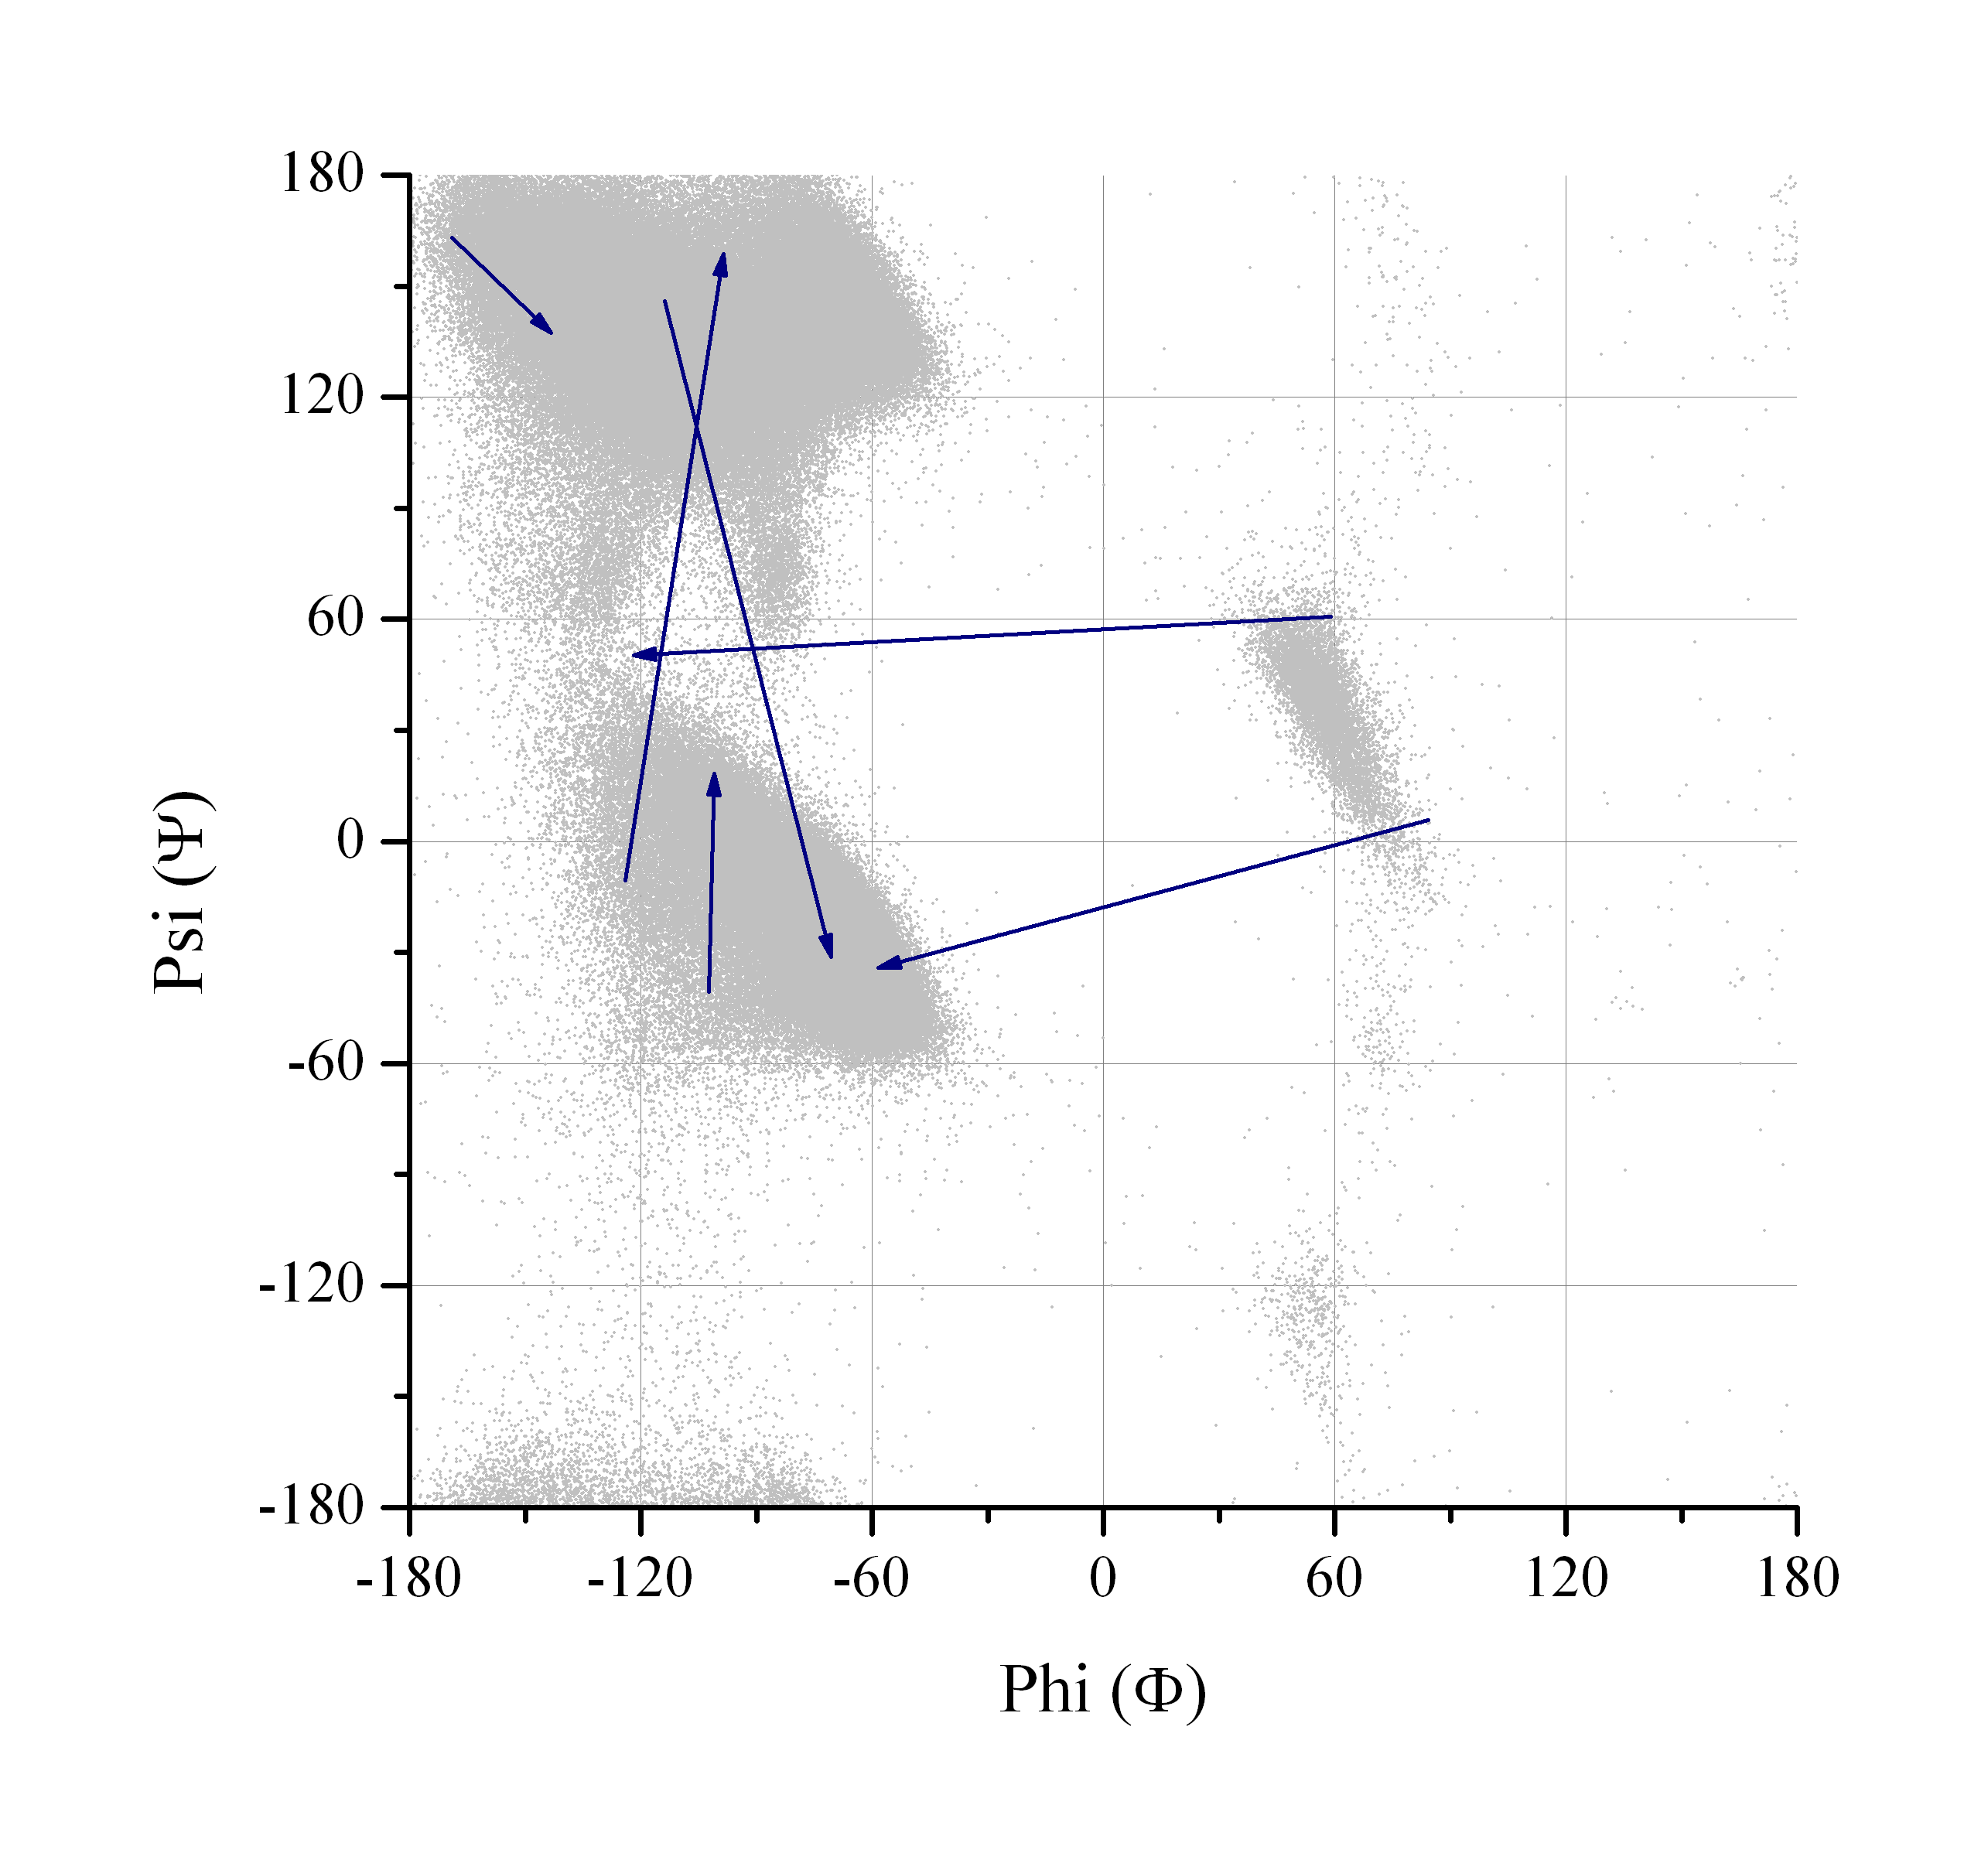
\includegraphics[width=0.45\textwidth]{07-CASP/high-t0345/worst_arms_pred_34_6_rama.png}}
\caption[The Ramachandran distributions for two example model structures]{This figure shows Ramachandran distribution deviations for two example model structures against the true \xray-derived structure as an arrow plot. The scatter data represents the data from \thothloopdb\ for all non-glycine and non-proline residues. Each arrow represents a single residue; pointing from the state used in the model to that of the \xray\ structure.}
\label{fig:casp:t0345_rama}
\end{center}
\end{figure}

Other predictions were of more poor quality. Figure \ref{fig:casp:t0345_poor} shows how a low \mainchain\ \crms\ structure, with an approximately-correct \mainchain\ path in Cartesian space, may be generated using incorrect torsions. For this example,   figure \ref{fig:casp:t0345_rama}-b shows that four torsion angles are in the incorrect regions of the Ramachandran map, but still within favoured regions.
As conformer generation is guided \emph{exclusively} under the influence of steric forces and \amberff\ torsional barriers, such structures are entirely unavoidable -- there is no reason for them to be disfavoured over the native. Interactions which guide the discrimination between such competing structures are likely to be formed using specific \sidechain\ conformations. These are essentially electrostatic and hydrophobic-burial interactions.
It is, therefore, the task of the higher-level energetic calculations to provide the discrimination. In these cases, assuming that multiple equally viable conformations were generated during the search, the \forcefield\ can be deemed to have failed in this discrimination.

\begin{figure}[hbtp]
\begin{center}
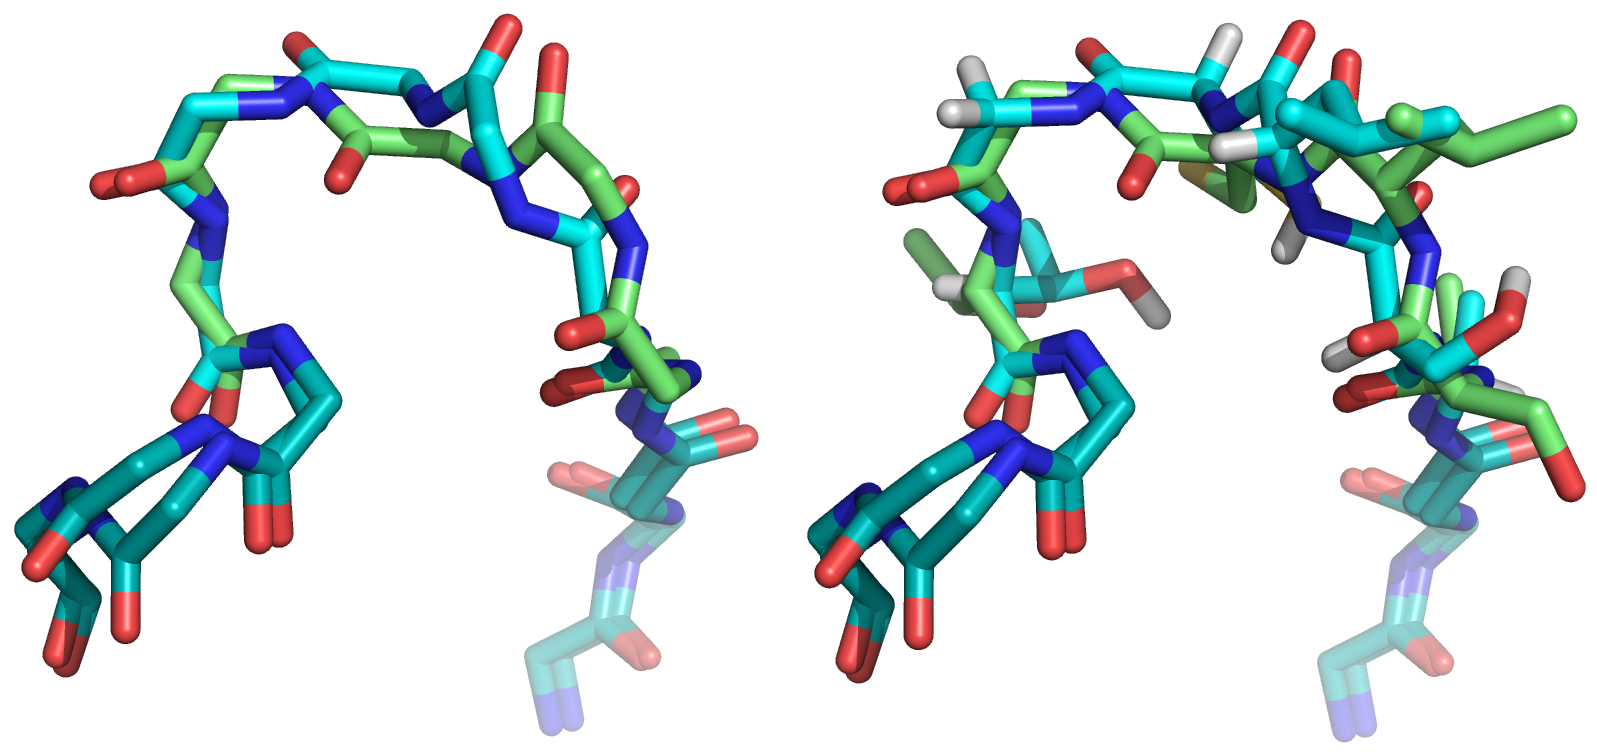
\includegraphics[width=0.8\textwidth]{07-CASP/high-t0345/worst_arms_pred_34_6.png}
\caption[The highest \arms\ prediction from T0345]{The highest \arms\  prediction from T0345; a \mer{6} loop beginning at residue Ala-34. The loop is shown on the left with no \sidechains\ for increased clarity. The crystal structure, model structure and anchor residues are shown in green, cyan and dark cyan respectively. Clear \mainchain\ torsional differences can be seen between the two structures.}
\label{fig:casp:t0345_poor}
\end{center}
\end{figure}

Finally, the prediction for the \mer{7} stretch from residue 94 was generated in an approximately mirrored conformation, shown in figure \ref{fig:casp:t0345_worst}-a. In this model, the overall \sidechain\ packing is poor, with a solvent-exposed leucine residue.
Hydrophobic residues can often be solvent-exposed in native structures, however, in this case there is a clear hydrophobic pocket in an appropriate location in the crystal structure, which was not utilised in the model. Although the loop follows approximately the correct path in space, the anchor residues are spaced widely, meaning that there is a more limited conformational space available to joined-conformations.
This structure should, therefore,  be deemed of poor quality. Figure \ref{fig:casp:t0345_worst}-b illustrates that it is not entirely the conformational search at fault in this case, as an alternative low \crms\ structure (1.0\AA\ \mainchain\ \crms) is visited during the conformational search, but is not selected as the best structure. Often when this occurs, as in this case, the atomic packing is not complete in the model, giving poor VDW energies. This is one of the specific problems with the use of standard molecular mechanics \forcefields.

\begin{figure}[hbtp]
\begin{center}
\subfigure[The model chosen as the lowest-energy state]{
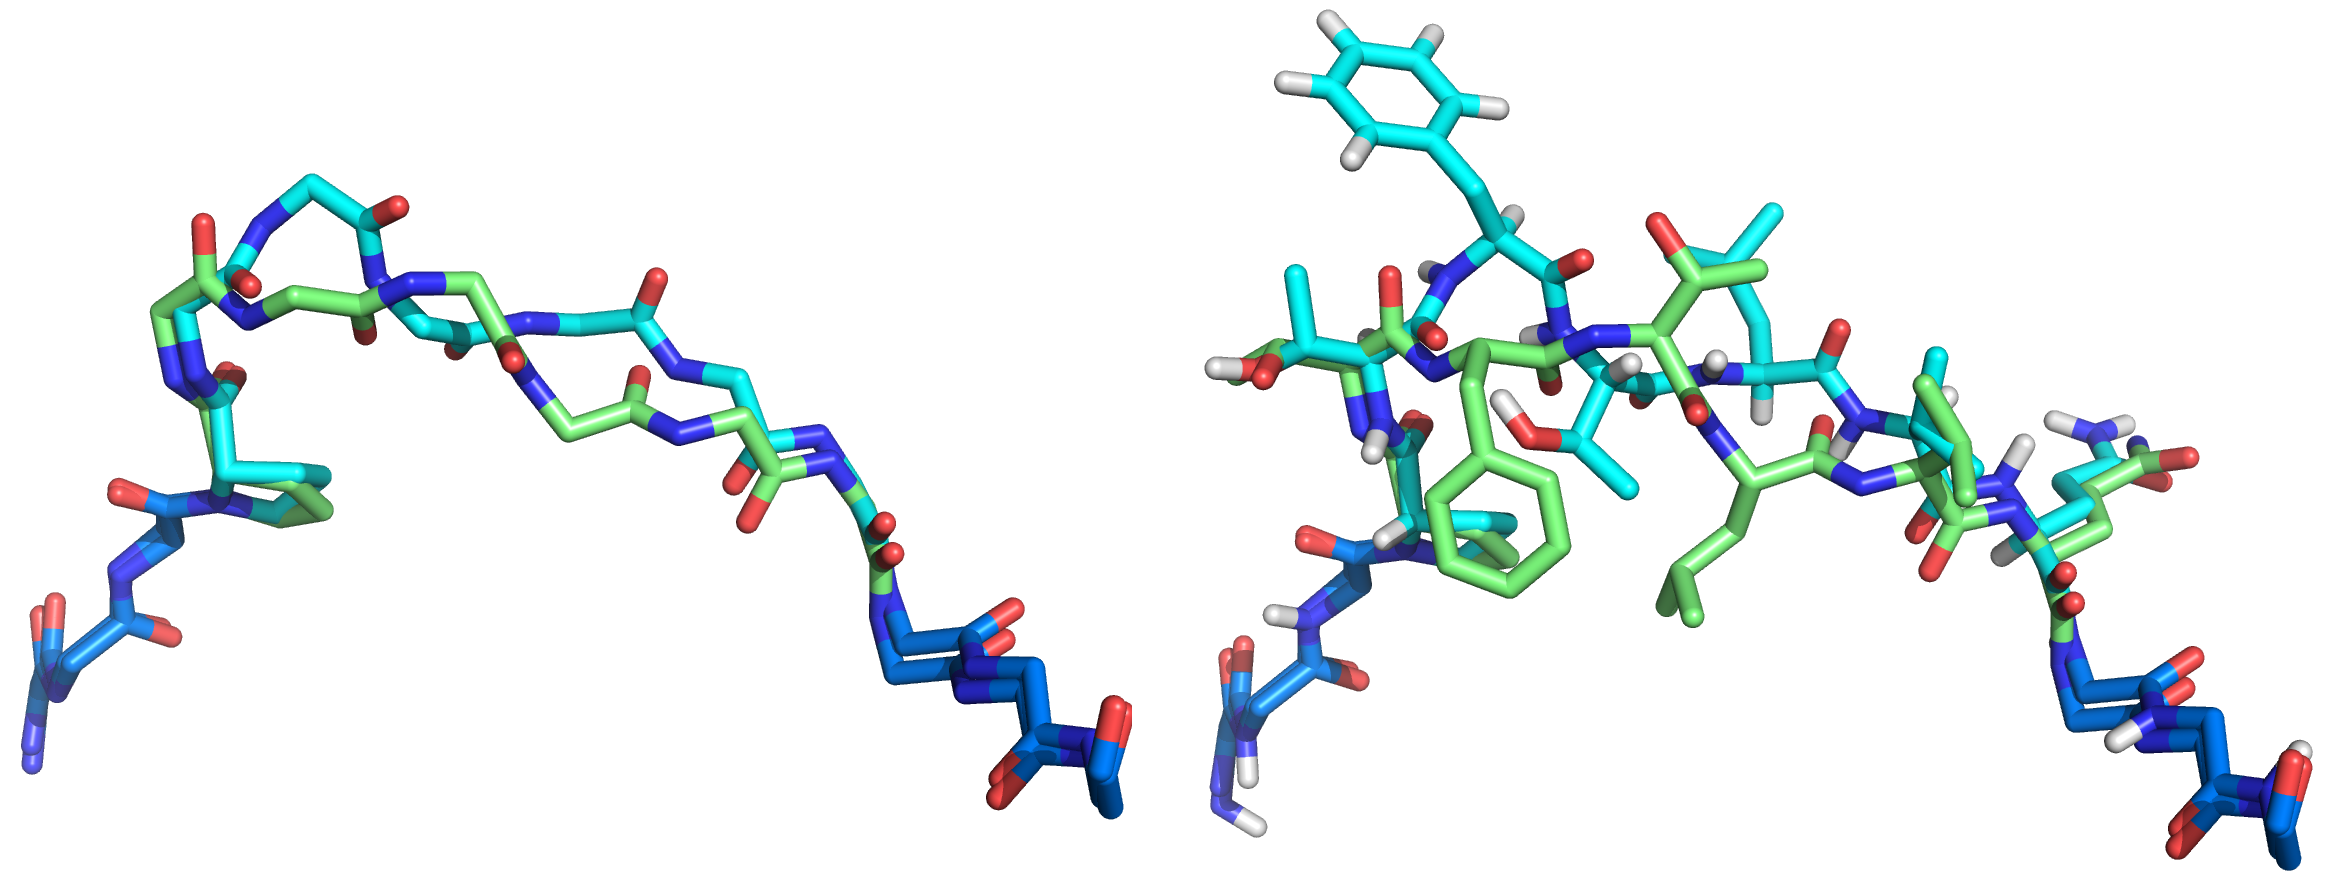
\includegraphics[width=0.95\textwidth]{07-CASP/high-t0345/poor_94_7.png}}
\subfigure[An alternative low-energy conformation visited during the search process]{
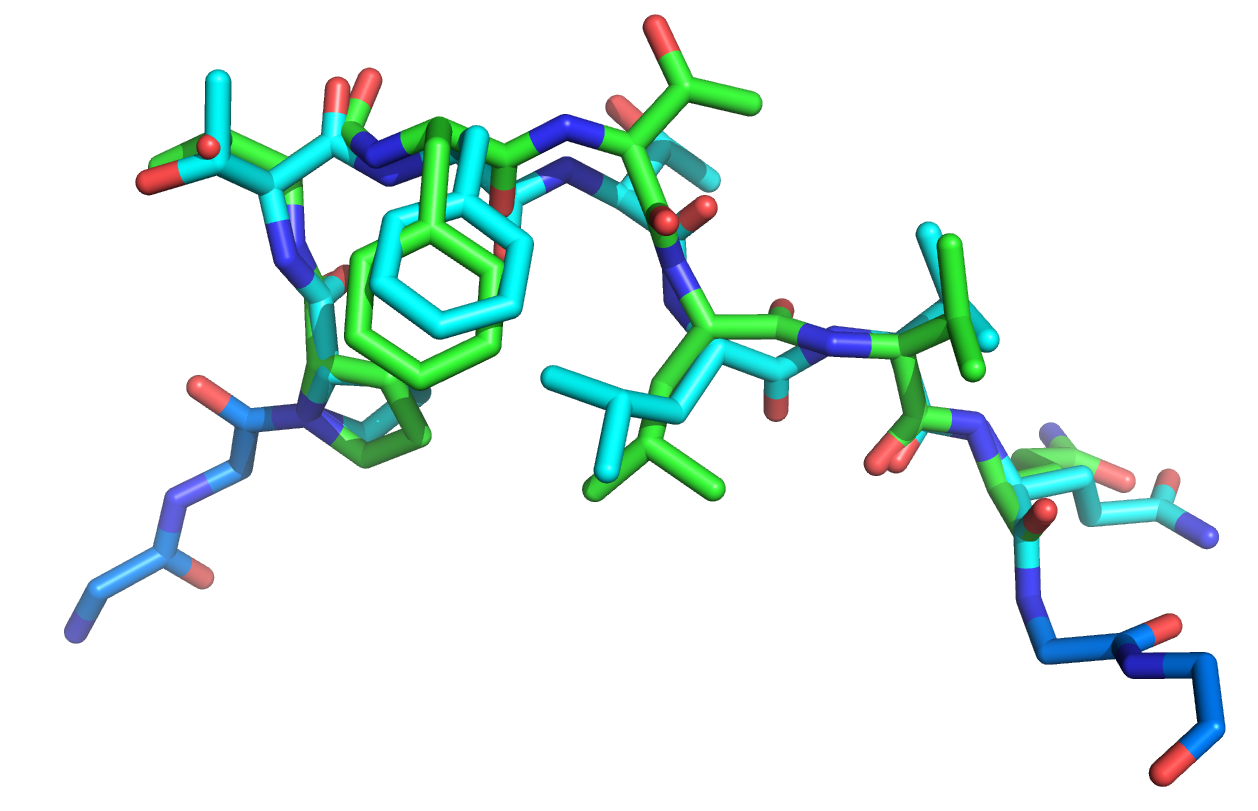
\includegraphics[width=0.75\textwidth]{07-CASP/high-t0345/poor_94_7_altstruc.png}}
\caption[One of the highest heavy-atom \crms\ prediction from T0345]{One of the highest (poorest) heavy-atom \crms\ predictions from T0345; a \mer{7} loop beginning at residue Pro-94. The loop is shown on the left of sub-figure a) with no \sidechains\ for increased clarity. The crystal structure, model structure and anchor residues are shown in green, cyan and dark cyan respectively. The model chosen as the single lowest visited energy-state is comparatively poor. It can, however, be seen that the underlying conformational search was successful as low \crms\ conformations are visited.\ }
\label{fig:casp:t0345_worst}
\end{center}
\end{figure}

As sequence identity falls into the medium-range, loop regions become comparatively longer to cover the increased uncertainty. There are, however, cases still of sufficient high-definition in anchor-regions to allow good predictions, such as in figure \ref{fig:casp:t0366_best}. In this example, one arginine \sidechain\ varies significantly from the \xray\ structure, but is fully solvent exposed and so intrinsically more difficult to predict. A second arginine is not resolved in the \xray\ structure, but of course, is defined in the model.

\begin{figure}[hbtp]
\begin{center}
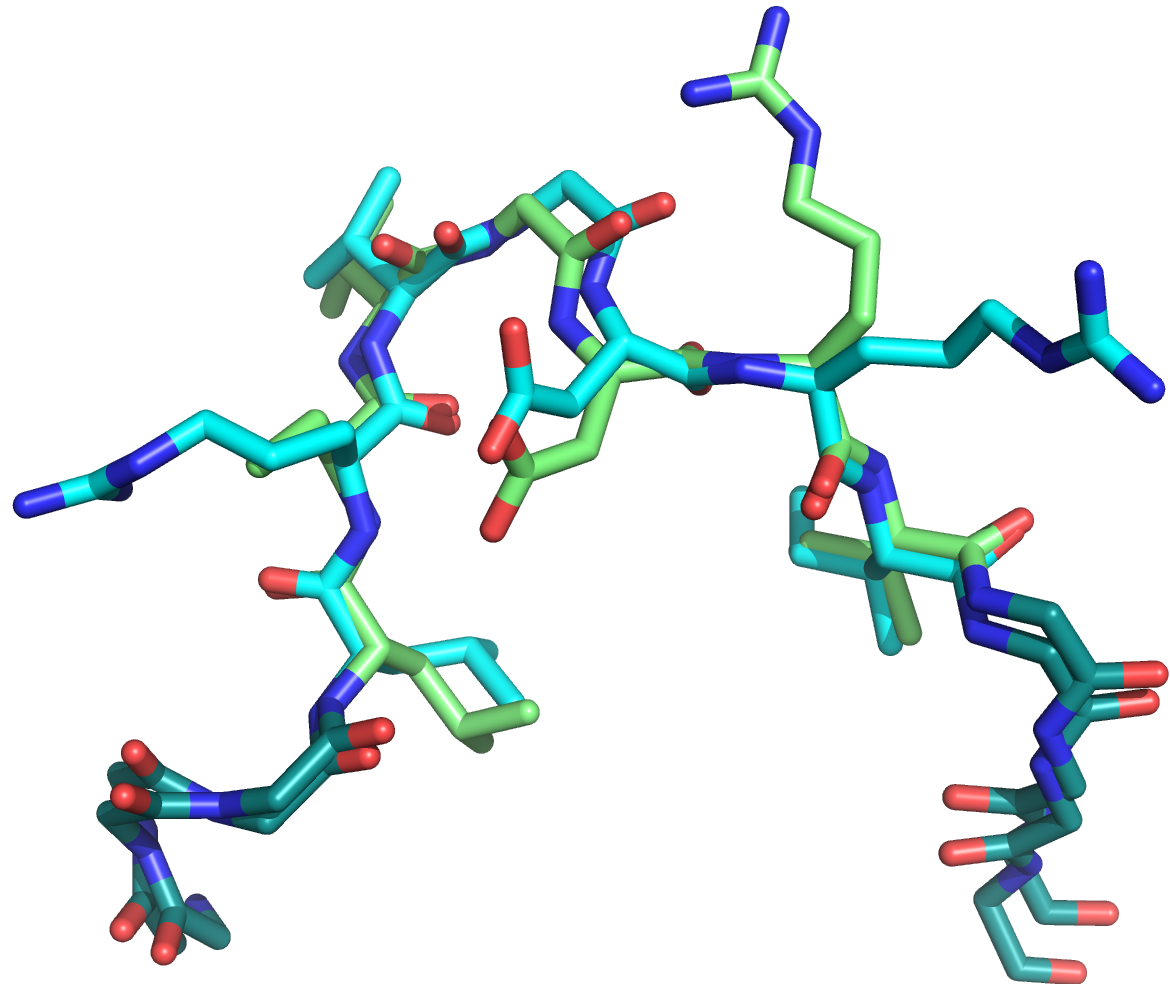
\includegraphics[width=0.75\textwidth]{07-CASP/med-t0366/33_7.png}
\caption[The best heavy-atom \crms\ prediction from T0366]{The best heavy-atom \crms\ prediction from T0366; a \mer{7} loop beginning at residue Leu-58. The crystal structure, model structure and anchor residues are shown in green, cyan and dark cyan respectively.  The \ca-\crms, Heavy-atom \crms\ and \arms\ are 1.50\AA, 2.12\AA\ and 9.63\degree\ respectively.}
\label{fig:casp:t0366_best}
\end{center}
\end{figure}

\subsection{Low Sequence-Identity}

To complete this results section, the low sequence-identity structures are considered next, where structural certainty in the rigid-body itself is low. In figure \ref{fig:casp:t0374_overext}, we clearly see that the \mainchain\ path diverges heavily within the rigid-core when compared to the \xray\ structure. Due to this, the prediction extends from an anchor residue which points in a direction incompatible with a correct prediction. Simply re-modelling loops is therefore insufficient at this level of sequence-identity. Clearly, in order to make any sensible predictions at this level, significant core re-modelling is also required.

\begin{figure}[hbtp]
\begin{center}
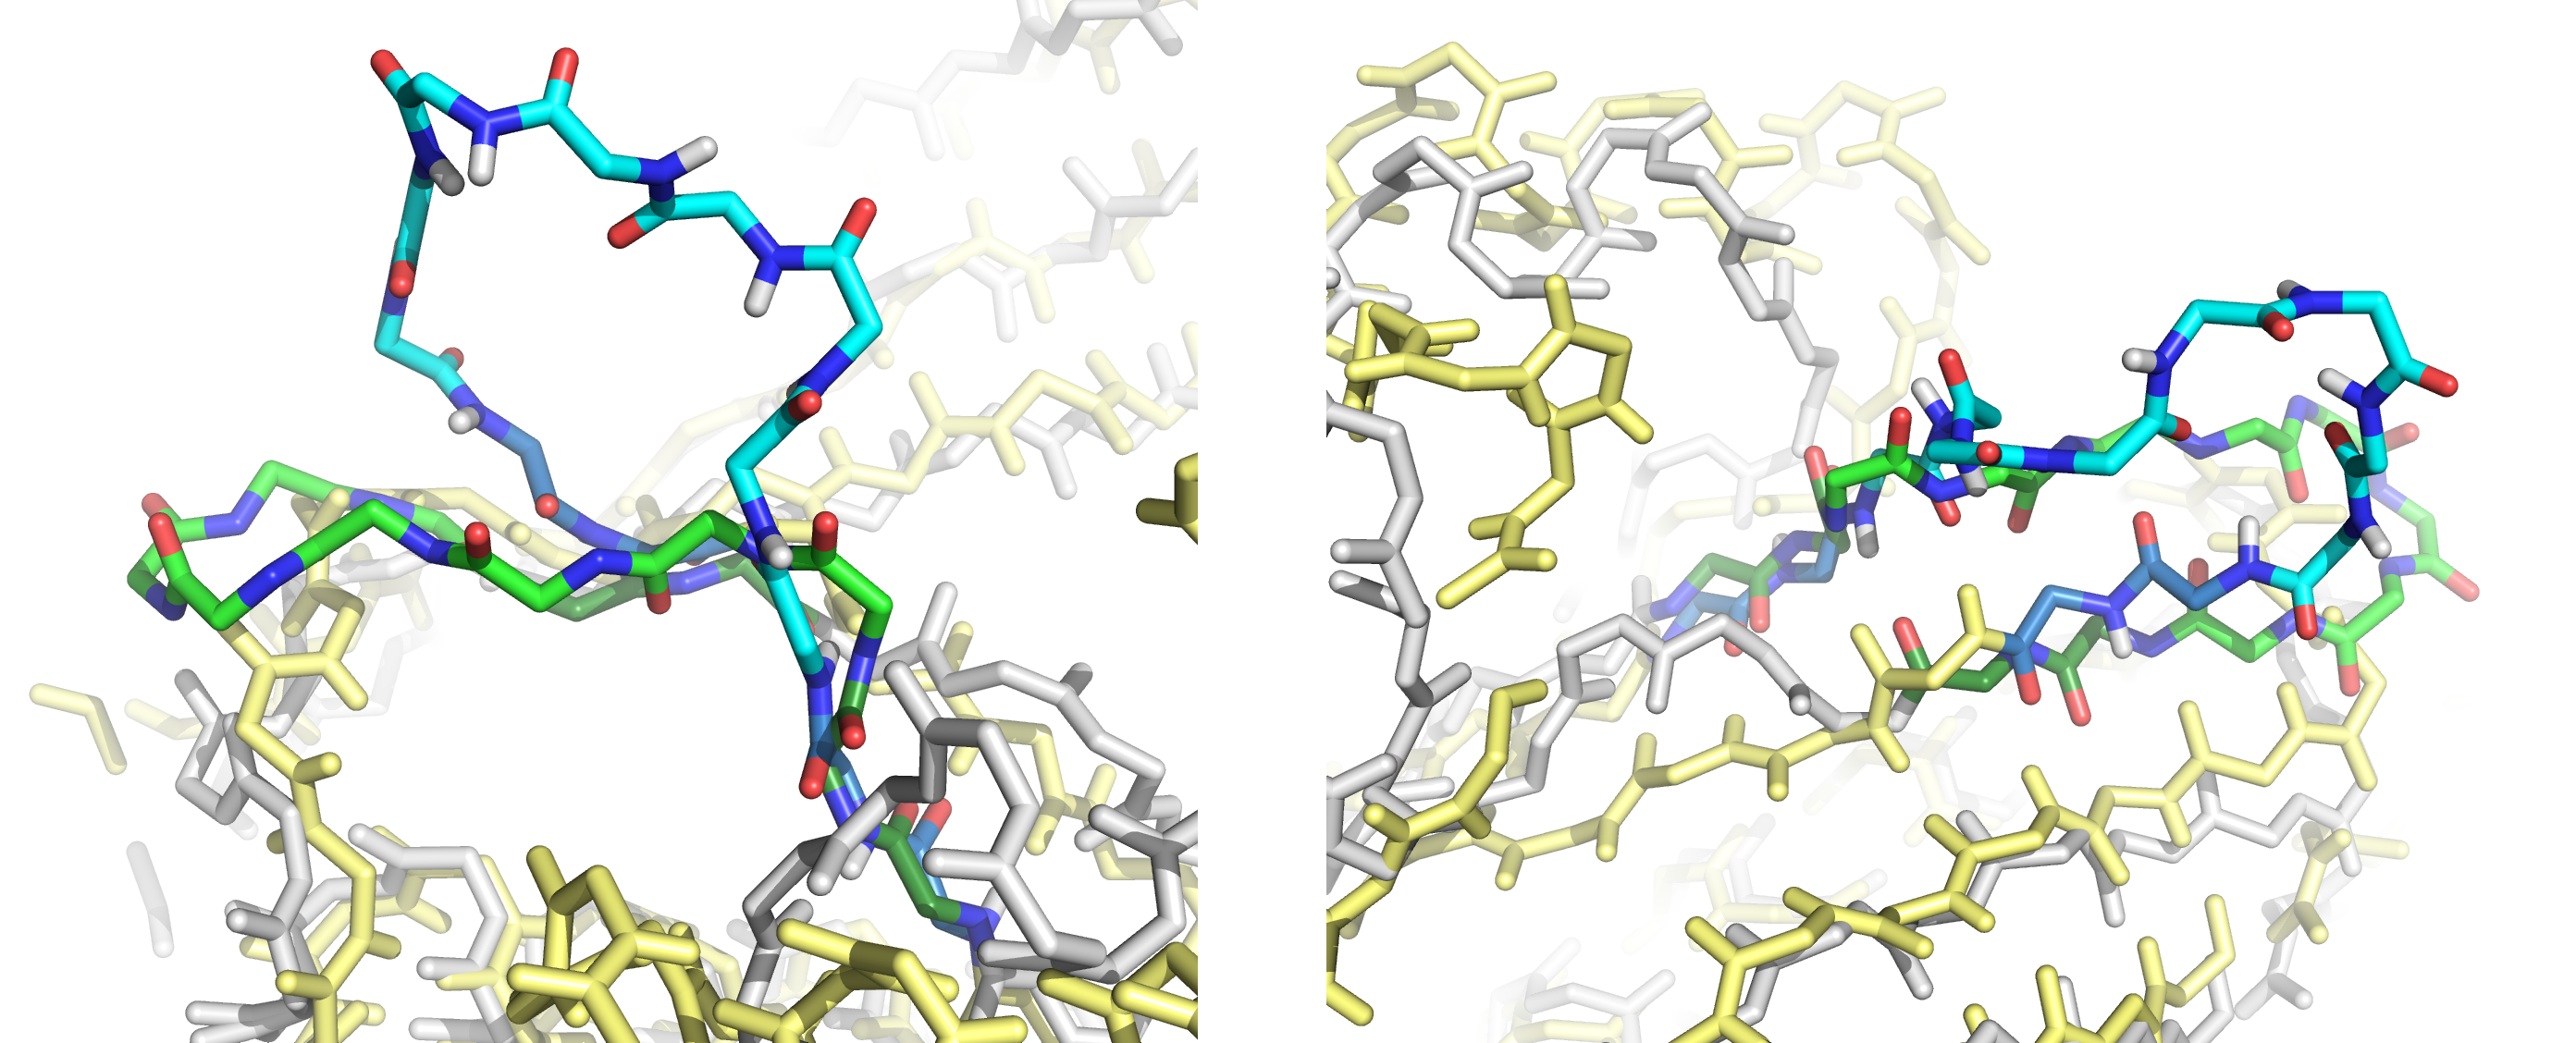
\includegraphics[width=0.99\textwidth]{07-CASP/low_t0374/t0374-68_8-overext.png}
\caption[Difficulties at low sequence-identity]{Difficulties at low sequence-identity. Here, two views of the same model for T0374 are shown with the \mer{8} loop prediction beginning at residue Tyr-68. The prediction can be seen to extend deep into solvent, making little surface-contact (left). A second observation is that the anchor regions are of poor structural correspondence between the two structures, with the \xray\ structure exhibiting a bulge in the \bsheet\ (right). The \xray\  structures, model loop, anchors and body are shown in green, dark green and grey respectively. The models loop, anchors and body are shown in cyan, dark blue and yellow respectively.}
\label{fig:casp:t0374_overext}
\end{center}
\end{figure}

\subsection{Other issues: Over-extension and Electrostatic Bias}

In addition to poor core correspondence, a second observation can be made from figure \ref{fig:casp:t0374_overext}, which is that the loop prediction extends far away from the protein body into solution. This also occurs for high sequence-identity structures and so the phenomenon is related to the \forcefield\ as opposed to anchor-residue uncertainty. Clearly, as this loop conformation was selected as the lowest-energy structure, the forcefield, as its stands, cannot discriminate against such structures. This difficulty is related to a second concern, which is that highly improbable \mainchain\ conformations were often found to be stabilised by  energetically favourable electrostatic interactions. These electrostatic interactions were both salt-bridges and hydrogen bonding interactions with charged partners. One such example is shown in figure \ref{fig:casp:t0379_salt}.

\begin{figure}[hbtp]
\begin{center}
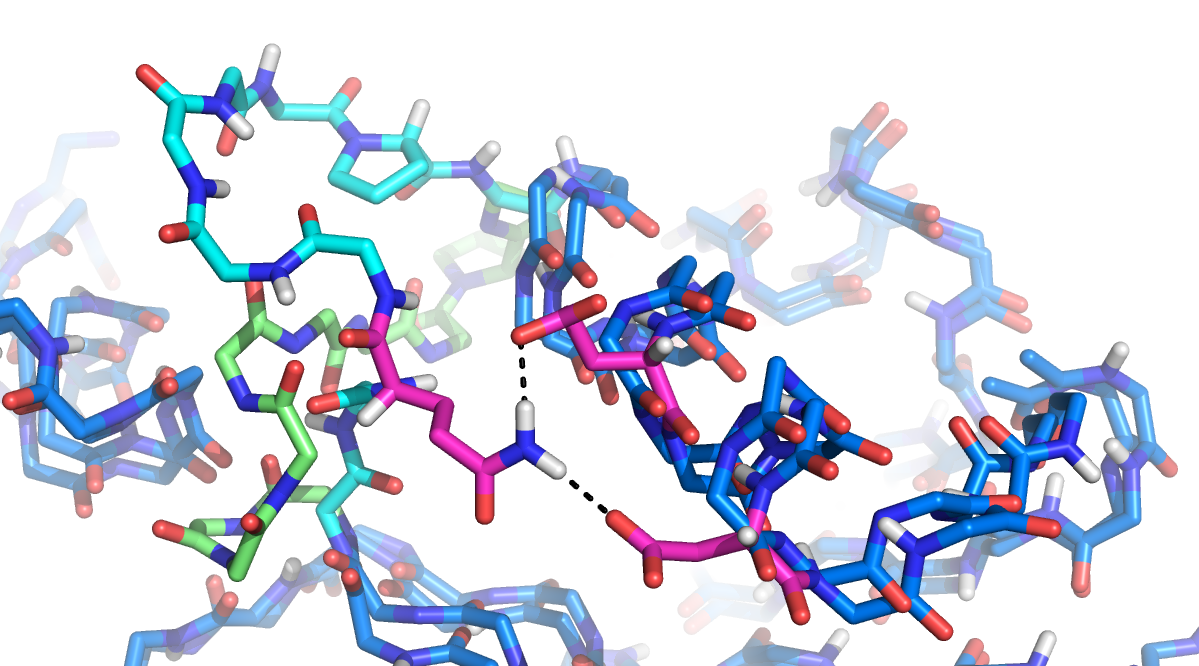
\includegraphics[width=0.9\textwidth]{07-CASP/salt-bridge/T0379_137_10-salt.png}
\caption[Difficulties at low sequence-identity]{Electrostatic-interactions can bias the conformation-selection process towards unpacked structures. In the example  from T0379, the protein cores, model loop, \xray\ structure loop and interacting residues are shown in blue, cyan, green and magenta respectively. The modelled Gln-141 is seen to interact via two strong electrostatic interactions to a pair of aspartic acid residues. This attracts the conformation away from the native-path and into solvent. The \forcefield\ is found to select poorly against these conformations, as the electrostatic and solvation terms are comparatively large compared to the VDW attractive term. }
\label{fig:casp:t0379_salt}
\end{center}
\end{figure}



\section{Discussion}

In this chapter, a qualitative overview of the results from the \casp-7\ assessment has been presented. In doing this, a number of important observations have been made, which are summarised separately in the following sub-sections. In addition to this, some other shortcomings within the logic used by \prearcus\ are outlined. Some of the more important aspects are used later to help improve the performance of \arcus; the specifics of which are discussed in depth in \mbox{chapter \ref{chapter:arcus}}.


\subsection{Over-powering Electrostatic Interactions}
\label{section:casp:salt_bridge_discussion}

A typical category of systematic error found in the models generated by \prearcus, was that a significant number of over-extended conformations were produced. A smaller number were then subsequently selected. In most of these selected overly-extended conformations, visual analysis revealed that one or more strong electrostatic interactions had been formed between two or more charged \sidechains. Each of these structures exhibited a strong electrostatic energy, over-shadowing other energetic components within the forcefield calculation. Further research into current literature on continuum electrostatics and solvation effects, revealed that this observation has been made previously by other groups in other contexts:

Firstly, during REMD simulations on TrpCage\cite{SIMULATION:SB1}, it was observed that solvent-exposed salt-bridges were over-stabilised; specifically in this case, the Asp9--Arg16 bridge. The \forcefield\ utilised in that work was the \amber\ '94 molecular mechanics forcefield\cite{FORCEFIELD:AMBER:94} and the GB/SA continuum solvation model\cite{COMPCHEM:Tsu2000}. Two further publications cited by this work describe further related observations. Specifically, that this forcefield combination both over-stabilises the folded states of proteins\cite{SIMULATION:SB1_32} and can also specifically over-stabilise \mbox{\al-helical} structures\cite{SIMULATION:SB1_33}.

Secondly, a paper analysing salt-bridge formation using \amber\ ff94 with the GB\superscript{HCT} implicit solvent model concluded that salt-bridges are too stable by around 3-4 \kcalmol\ in proteins containing ionisable groups\cite{SIMULATION:SB2}. Thus, they designed a minor forcefield adjustment, whereby the radius of hydrogen atoms which are bonded to charged nitrogen atoms was reduced from 1.3\AA\ to 1.1\AA.
In their simulations, this empirical fix was shown to improve the correlation between various distance-variation measurements  when compared to those in explicit solvent (\textsc{Tip3P}).

Most GB models are parametised and validated against their ability to reproduce the data generated using the Poisson Boltzman continuum electrostatic approximation\cite{FORCEFIELD:Qui1997,FORCEFIELD:GB:ADVANCES:B,FORCEFIELD:SGB,COMPCHEM:Tsu2000}. A recent paper however develops the continuum solvent model AGBNP which takes the view that the errors introduced by the continuum approximation far outweigh those introduced in the GB model itself. With that in mind, their Born radii and atomic surface area parameters are parametised to reproduce experimental and explicit solvent derived data, rather than Poisson Boltzman-derived values. Some impressive results are generated during their simulations -- the method was also shown to have discriminating power when applied to the \plop\ loop decoy-set\cite{METHOD:Plop}; in over 90\% of the test cases, a structure of less than 2.0\AA\ RMSD was selected by the forcefield. Such \forcefield\ enhancements, although not implemented in this work, would likely be excellent future directions for \arcus\ development.

A more immediate solution, to the more fundamental problem of the generation of over-extended conformations, is simply to filter them out earlier in the search process. Such filtering is computationally cheap and would increase efficiency, as such conformations will no longer enter refinement. There should also be an increase in predictive performance as native loop conformations are observed to extend significantly into solvent in rare cases\cite{METHOD:Plop}.

\subsection{Anchor-Residue Placement Quality}

It is observed here that, unsurprisingly, the conformation of the loop anchor-residues has an overwhelming influence on surface-loop predictions. As a result of this, their exact placement is of paramount importance. In this assessment, sequence divergence and server-model similarity were used to influence the length of the loop regions chosen for refinement. Obviously, as sequence-identity in the vicinity of the surface-loop falls, the exact placement of the anchor residues will become less and less certain. In medium sequence-identity targets, the size of loop region can be increased slightly to include remodelling of the closest anchor residues. Such an extension must take into account that increasing the loop length by just one residue, greatly increases the magnitude of the simulation. 

Figure \ref{fig:casp:t0374_overext}
was used to show that at below 25\% sequence-identity, anchor residue placement accuracy is so low that loop-refinement is essentially irrelevant -- no matter how detailed the refinement, it is guaranteed to be incorrect. In essence, the rigid-body approximation ceases to be effective below medium sequence-identity and therefore should not be used in combination with \arcus\ --  unless in conjunction with a complementary core-remodelling algorithm. It should be stated that such calculations would be extremely computationally expensive, as loop predictions would need to be made per core-model. 




\subsection{Side-chain Packing}

In some cases, the \sidechain\ packing of the lowest energy structure, was found to be sub-optimal. What is certainly true is that the packing algorithm used by \prearcus, although performing sensible steric tests, was overly reliant on pure random-perturbation and made no use of the known probability distributions of potential rotamer states. It is, however, known that the \mainchain\ \phipsi\ angle-pairs are of critical importance in determining the likelihood of different competing \sidechain\ conformations\cite{METHOD:SCWRL_1}.
The use of backbone-dependent rotamer libraries is likely to improve the performance of \arcus.
In addition to this, the implementation of a deterministic rotamer-packing algorithm would also be beneficial.
\subsection{Parametisation} 
\prearcus\ uses a multitude of cut-offs and parameters in an attempt to increase efficiency. The first difficulty is that, as there are so many of these parameters, global parametisation is impossible. Each parameter is therefore optimised in isolation, sometimes somewhat arbitrarily, based upon typical observed values from a small number of test cases. The other general difficulty with the use of fixed cut-offs is that their optimal magnitude can change dependent on the current system. For example, the stage 2 total steric energy is actually  dependent on the number of atoms in the local vicinity and on whether there are clashes in the rigid-body itself. 

Further development, therefore, requires the reevaluation of the filtering system. Fixed parameters should be replaced with adaptive methods wherever possible. This could involve retaining the top $x\%$ of structures under given criteria, discarding structures which are of poorer quality than the best generated to that point, or the use of dynamic cut-offs which change in response to measurements obtained from conformations as they are produced. Where this is not possible, cut-offs should be tightly parametised using high quality experimental data. It is also important to choose filters with cut-offs that do not vary significantly with differing protein contexts or with loop length.

 \subsection{The Torsional Minimisation}
 \label{section:casp:torsionalMinimisation}

One further observation, which is difficult to describe diagrammatically, can be effectively described  anecdotally. It was found that, as the loop-rejoin-force is required to be of reasonable strength to perform its function, the minimisation was capable of allowing \mainchain\ torsional barriers to be crossed during restraint satisfaction. Some final \mainchain\ torsions were consequently found to be on the extreme borders of allowable Ramachandran regions. In addition to this, for the same reason,  during energy minimisation large Cartesian movements were sometimes seen which affected the entire conformer. 

In light of these more extreme movements, if more detailed structural filters are to be employed, then additional \mainchain\ Cartesian restraints may be required. These would ensure that the structure did not deviate very significantly during the minimisation. This would ensure that the starting conformation, which passed all structural filters, does not often make transitions to conformational-states which do not pass. 

\subsection{Summary}

In this chapter we have seen that, with some caveats, \prearcus\ is capable of making  excellent predictions. Indeed, when considering the model-structure illustrations presented in both figures \ref{fig:casp:t0345_best} and \ref{fig:casp:t0366_best}, it should be noted that the observed \mainchain\ deviations are of comparable magnitude to the largest seen in figure \ref{fig:casp:crystalsimilarity},  which illustrated the observed differences between same-sequence \xray-structures.
For real-world interpretation of loop structure, these predictions could be used to make atomic-resolution measurements
of genuine use.

Where loop prediction fails, plausible explanations can usually be given, thus attempts to rectify these problems can be made. For example, the use of filtering procedures  in the early stages of the conformational search to remove over-extended conformations is trivial to implement.
Other aspects such as improved \sidechain\ packing require significant additional implementation, but should greatly improve predictive performance.
Finally, problems with \forcefield\ performance are not directly related to \prearcus\ itself, as stages 1 and 2 of the conformational search are entirely  \forcefield\ independent. The choice of \forcefield\ is, however, important as a determinant of ultimate prediction quality in stage 3.\ Therefore, this should, be considered carefully.

A significant remaining issue is prediction at low sequence-identity. At this level, the quality of the protein-core prediction is so low, it essentially renders \prearcus\ useless. To tackle this level of target other algorithms must be employed which refine the structure as a whole. Such tasks are, therefore, fundamentally beyond the scope of \arcus\ as a comparative-modelling tool.

